\chapter{The Method of Types and Moment Conditioning}
\label{ch:types}

\section{Counting as a theory of probability}

Boltzmann's derivation of 1877~\cite{boltzmann1877} counted the ways of distributing molecules among cells of phase space. Eighty years later Sanov~\cite{sanov1957} proved the large deviation theorem for empirical distributions, and Csisz\'ar and K\"orner~\cite{csiszarkorner2011} made the counting into a systematic method, the method of types, which gives exact, nonasymptotic bounds for the probabilities of empirical distributions on finite alphabets. The method is elementary. It proves Sanov's theorem, the conditional limit theorem and Stein's lemma on finite alphabets, and it explains why conditioning a large system on its macroscopic moments produces the exponential families of statistical mechanics.

\section{Types and type classes}

Let $\mathcal{X} = \{1,\dots,m\}$ and $x = (x_1,\dots,x_n)\in\mathcal{X}^n$. The type of $x$ is its empirical distribution $Q_x(a) = \frac1n\#\{i:x_i = a\}$. Let $\mathcal{P}_n$ be the set of types of sequences of length $n$, and for $Q\in\mathcal{P}_n$ let $T(Q) = \{x:Q_x = Q\}$ be its type class. For independent random variables $X_1,X_2,\dots$ with values in $\mathcal{X}$, write $L_n$ for the type of $(X_1,\dots,X_n)$, the empirical measure. Logarithms are natural, $H(Q) = -\sum_aQ(a)\log Q(a)$ is the Shannon entropy, and $\KL(Q\|P) = \sum_aQ(a)\log\frac{Q(a)}{P(a)}$ is the relative entropy, with $0\log0 = 0$ and $\KL(Q\|P) = \infty$ unless $Q$ vanishes wherever $P$ does.

\begin{theorem}[Type counting]
\label{thm:typecount}
\begin{enumerate}
\item $|\mathcal{P}_n|\leq(n+1)^m$.
\item For any law $P$ on $\mathcal{X}$ and $x\in T(Q)$, $P^n(x) = \exp\big(-n(H(Q)+\KL(Q\|P))\big)$.
\item For $Q\in\mathcal{P}_n$, $(n+1)^{-m}e^{nH(Q)}\leq|T(Q)|\leq e^{nH(Q)}$.
\item For $Q\in\mathcal{P}_n$ and any $P$, $(n+1)^{-m}e^{-n\KL(Q\|P)}\leq P^n(T(Q))\leq e^{-n\KL(Q\|P)}$.
\end{enumerate}
\end{theorem}

\begin{proof}
(1) Each coordinate $nQ(a)$ takes one of $n+1$ values. (2) $P^n(x) = \prod_aP(a)^{nQ(a)} = \exp(n\sum_aQ(a)\log P(a))$, and $\sum_aQ\log P = -H(Q)-\KL(Q\|P)$. (3) By (2) with $P = Q$, every sequence in $T(Q)$ has $Q^n$ probability $e^{-nH(Q)}$, so $1\geq Q^n(T(Q)) = |T(Q)|e^{-nH(Q)}$. For the lower bound we show that $T(Q)$ is the most probable type class under $Q^n$: for $Q'\in\mathcal{P}_n$,
\[
\begin{aligned}\frac{Q^n(T(Q))}{Q^n(T(Q'))} &= \prod_a\frac{(nQ'(a))!}{(nQ(a))!}\,Q(a)^{n(Q(a)-Q'(a))}\\ &\geq\prod_a(nQ(a))^{n(Q'(a)-Q(a))}Q(a)^{n(Q(a)-Q'(a))} = 1,\end{aligned}
\]
using $k!/l!\geq l^{k-l}$ and $\sum_aQ'(a) = \sum_aQ(a)$. Since there are at most $(n+1)^m$ types, $Q^n(T(Q))\geq(n+1)^{-m}$, and $|T(Q)| = Q^n(T(Q))e^{nH(Q)}$. (4) Multiply (3) by the common probability $e^{-n(H(Q)+\KL(Q\|P))}$ from (2).
\end{proof}

Part (3) is Boltzmann's $\log W = nH$ with a polynomial correction, and part (4) is the exact form of Sanov's theorem~\cite{sanov1957} (Theorem~\ref{thm:sanov}): the probability of observing the type $Q$ when the truth is $P$ decays at the rate $\KL(Q\|P)$, with no error term beyond a polynomial factor. The bounds are those of Csisz\'ar and K\"orner~\cite{csiszarkorner2011} and of Cover and Thomas~\cite[Section~11.1]{covertomas}.

Figure~\ref{fig:types} shows the types as points of the probability simplex, superimposed on the contours of $\KL(Q\|P)$. Types near $P$ are exponentially more likely than distant ones, and the rate is read off the contour on which a type lies.

\begin{figure}[t]
\centering
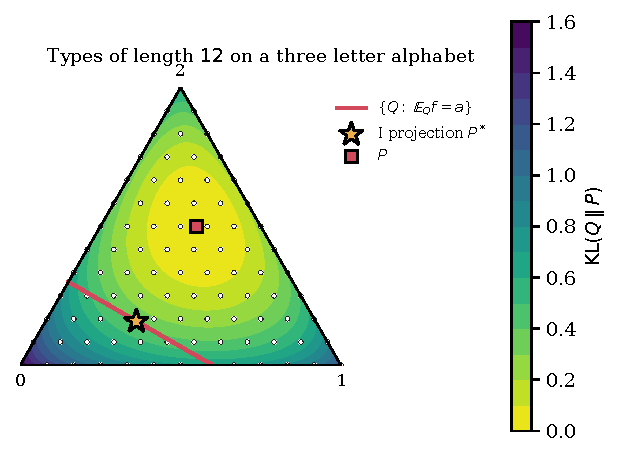
\includegraphics[width=0.78\textwidth]{types_simplex}
\caption{Types of length $12$ on $\{0,1,2\}$ (the $91$ white points, the lattice points of the simplex with spacing $1/12$) over the contours of $\KL(Q\,\|\,P)$ with $P=(0.2,0.3,0.5)$ (square). The corners of the triangle are the point masses at $0$ (lower left), $1$ (lower right) and $2$ (top). The straight line is the linear family $\{Q:\E_Qf=0.6\}$ for $f(x)=x$, and the star is its I projection $P^*\approx(0.559,0.283,0.159)$, an exponential tilt of $P$. No type of length $12$ lies on the line, because $12\,\E_Qf = 7.2$ is not an integer, so the line passes between the points.}
\label{fig:types}
\end{figure}

\section{The I projection and the Pythagorean theorem}

\begin{definition}
Let $E$ be a closed convex set of laws on $\mathcal{X}$ and $P$ a law with full support such that $\KL(Q\|P)<\infty$ for some $Q\in E$. The I projection of $P$ onto $E$ is the unique $P^*\in E$ minimizing $\KL(Q\|P)$ over $E$.
\end{definition}

Existence follows from compactness and lower semicontinuity, uniqueness from strict convexity of $Q\mapsto\KL(Q\|P)$.

\begin{theorem}[Csisz\'ar's Pythagorean inequality]
\label{thm:pythagoras}
Let $P^*$ be the I projection of $P$ onto the closed convex set $E$. Then for every $Q\in E$,
\[
\KL(Q\,\|\,P)\geq\KL(Q\,\|\,P^*)+\KL(P^*\,\|\,P).
\]
If $E$ is a linear family $\{Q:\E_Qf_j = a_j,\ j = 1,\dots,r\}$, equality holds for every $Q\in E$. If in addition $P^*$ has full support, $P^*$ is the exponential tilt
\[
P^*(x) = \frac{P(x)\exp\big(\sum_j\lambda_jf_j(x)\big)}{Z(\lambda)},
\]
with $\lambda$ chosen so that the moment constraints hold.
\end{theorem}

\begin{proof}
For $Q\in E$ and $t\in[0,1]$, $Q_t = (1-t)P^*+tQ\in E$, so $\phi(t) = \KL(Q_t\|P)$ is minimized at $t = 0$. First, $Q\ll P^*$. If $Q(x_0)>0 = P^*(x_0)$ for some $x_0$, the term $Q_t(x_0)\log\frac{Q_t(x_0)}{P(x_0)}$ of $\phi$ has a derivative that tends to $-\infty$ as $t\downarrow0$, while the derivative of every other term is bounded above near $0$, so that $\phi(t)<\phi(0)$ for small $t>0$, a contradiction. All sums below therefore run over the support of $P^*$, and the right derivative of $\phi$ at $0$ is nonnegative:
\[
\phi'(0^+) = \sum_x\big(Q(x)-P^*(x)\big)\log\frac{P^*(x)}{P(x)}\geq0,
\]
where the constant produced by differentiating $q\log q$ drops out because $\sum_x(Q(x)-P^*(x)) = 0$. A direct computation shows that
\[
\begin{aligned}\KL(Q\|P)-\KL(Q\|P^*)-\KL(P^*\|P) &= \sum_xQ\log\frac{P^*}{P}-\sum_xP^*\log\frac{P^*}{P}\\ &= \phi'(0^+),\end{aligned}
\]
which proves the inequality. For a linear family, $Q_t\in E$ also for small negative $t$, because the constraints are affine in $t$ and $Q_t\geq0$ since $Q\ll P^*$. Then $\phi$ is differentiable at $0$ and minimized there, so $\phi'(0) = 0$ and equality holds. Now let $P^*$ have full support. Then $P^*+t\nu\in E$ for small $|t|$ and every signed measure $\nu$ with total mass zero and $\sum_x\nu(x)f_j(x) = 0$ for all $j$, and the same argument gives $\sum_x\nu(x)\log\frac{P^*(x)}{P(x)} = 0$. So $\log(P^*/P)$ is orthogonal to all such $\nu$, hence lies in the span of $1,f_1,\dots,f_r$, which is the exponential form.
\end{proof}

The theorem is due to Csisz\'ar~\cite[Theorem~2.2]{csiszar1975}, who also proved the exponential form~\cite[Theorem~3.1]{csiszar1975}. It says that relative entropy behaves like squared Euclidean distance, with exponential families playing the role of orthogonal complements of linear families. Two consequences are used repeatedly. First, maximum likelihood in the exponential family $\{P_\lambda\}$ and I projection onto the linear family of laws with the observed moments are dual problems with the same solution: a maximizer of the log likelihood per observation, $\sum_j\lambda_ja_j-\log Z(\lambda)$ plus a constant, where $a_j$ is the observed mean of $f_j$, satisfies $\E_{P_\lambda}f_j = a_j$, so $P_\lambda$ lies in the linear family, and a tilt that lies in the linear family is its I projection~\cite[Theorem~3.1]{csiszar1975}. This duality makes the maximum entropy principle~\cite{jaynes1957} and maximum likelihood two faces of one computation. Second, iterative proportional fitting~\cite{demingstephan1940} and Sinkhorn's algorithm~\cite{sinkhorn1964} of Chapter~\ref{ch:gbc} are alternating I projections onto two linear families, the laws on a product alphabet with a given first marginal $r$ and those with a given second marginal $c$. Start from a law $\pi_0 = P$ with full support, and let $\pi_{t+1}$ be the I projection of $\pi_t$ onto the first family when $t$ is even and onto the second when $t$ is odd; the I projection onto a marginal constraint rescales the rows, or the columns, of $\pi_t$. The two families intersect, since both contain $r\otimes c$, and Csisz\'ar~\cite[Theorem~3.2]{csiszar1975} showed that $\pi_t$ then converges to the I projection $\pi^*$ of $P$ onto the intersection. Because $\pi^*$ lies in both families, the Pythagorean identity gives $\KL(\pi^*\|\pi_t) = \KL(\pi^*\|\pi_{t+1})+\KL(\pi_{t+1}\|\pi_t)$ at every step, so that relative entropy to $\pi^*$ descends monotonically (Exercise~\ref{ex:ipf}). Chapter~\ref{ch:gbc} proves the convergence of Sinkhorn's algorithm by another route, Birkhoff's contraction in Hilbert's projective metric.

\section{The conditional limit theorem}

\begin{theorem}[Conditional limit theorem]
\label{thm:conditional}
Let $X_1,X_2,\dots$ be independent with law $P$ of full support on $\mathcal{X}$ and let $E$ be a closed convex set of laws with I projection $P^*$. Suppose that for all large $n$ the set $E$ contains a type $Q_n\in\mathcal{P}_n$, and that $Q_n\to P^*$. Then $\P(L_n\in E)>0$ for all large $n$, and for every fixed $k$,
\[
\mathrm{Law}\big(X_1,\dots,X_k\,\big|\,L_n\in E\big)\longrightarrow(P^*)^{\otimes k}.
\]
Moreover $\P(\KL(L_n\|P^*)>\delta\mid L_n\in E)\to0$ exponentially fast for each $\delta>0$.
\end{theorem}

\begin{proof}
By the Pythagorean inequality of Theorem~\ref{thm:pythagoras}, every type $Q\in E$ with $\KL(Q\|P^*)>\delta$ has $\KL(Q\|P)\geq\KL(P^*\|P)+\delta$. By Theorem~\ref{thm:typecount}, the total probability of such types is at most $(n+1)^me^{-n(\KL(P^*\|P)+\delta)}$. Since $Q_n\to P^*$ and $P$ has full support, $\KL(Q_n\|P)\to\KL(P^*\|P)$, and hence $\P(L_n\in E)\geq\P(L_n = Q_n)\geq(n+1)^{-m}e^{-n(\KL(P^*\|P)+\delta/2)}$ for large $n$. The ratio is at most $(n+1)^{2m}e^{-n\delta/2}$, which is the second claim. For the first, let $Q\in E\cap\mathcal{P}_n$. Conditionally on $L_n = Q$ the sequence is uniform on the type class, so the law of $(X_1,\dots,X_k)$ is that of sampling without replacement from an urn with composition $nQ$. Sampling with replacement gives $Q^{\otimes k}$, and the two laws differ by at most the probability that $k$ draws with replacement from $n$ balls include a repeat, which is at most $k(k-1)/(2n)$. This is the bound of Diaconis and Freedman~\cite{diaconisfreedman1980}, with total variation taken as the supremum over events. Total variation is subadditive for products, so $Q^{\otimes k}$ is within $k\,\mathrm{TV}(Q,P^*)$ of $(P^*)^{\otimes k}$, and Pinsker's inequality~\cite[Lemma~11.6.1]{covertomas} gives $\mathrm{TV}(Q,P^*)\leq\sqrt{\KL(Q\|P^*)/2}$. Averaging over the conditional law of the type, the law of $(X_1,\dots,X_k)$ given $L_n\in E$ is within $k(k-1)/(2n)+k\sqrt{\delta/2}+(n+1)^{2m}e^{-n\delta/2}$ of $(P^*)^{\otimes k}$ in total variation, for every $\delta>0$, and the claim follows by letting $n\to\infty$ and then $\delta\downarrow0$.
\end{proof}

This is the conditional limit theorem of Van Campenhout and Cover~\cite{vancampenhoutcover1981} and Csisz\'ar~\cite{csiszar1984}, proved by types as in Cover and Thomas~\cite[Section~11.6]{covertomas}. Theorem~\ref{thm:gibbs_conditioning} proves Gibbs conditioning for one inequality constraint on the mean of a single function. The theorem above allows any closed convex set of laws, such as several moment constraints at once, and its proof gives explicit bounds: an exponential rate for the concentration of the type and the error $k(k-1)/(2n)$ from the urn. The proof makes visible why the limit is an exponential tilt: conditioning on a macroscopic constraint selects the most probable type compatible with it, and the most probable type is the I projection, which is a tilt when the constraint is linear by Theorem~\ref{thm:pythagoras}. The urn step is de Finetti's theorem for finite sequences~\cite{diaconisfreedman1980} (Theorem~\ref{thm:diaconis_freedman}): conditionally on its type, a sequence is exchangeable and its short marginals are nearly independent.

The hypothesis on $E$ holds whenever $E$ has nonempty interior in the simplex: a ball around an interior point contains a type for every large $n$, and every point of a convex set with interior, in particular $P^*$, is a limit of interior points. This covers the inequality constraints $\{Q:\E_Q\varepsilon\leq a\}$ of Theorem~\ref{thm:gibbs_conditioning} and shells $\{a\leq\E_Qf\leq a+\delta\}$ of positive width. It also holds for an equality constraint $\{Q:\E_Qf = a\}$ when $f$ is integer valued and $P^*$ has full support, along the $n$ for which $E$ contains a type at all: the count vectors of types in $E$ are the integer points of an affine subspace that contains $nP^*$, they form a translate of a lattice, and so one of them lies within a bounded distance of $nP^*$. The proof then gives the conclusion along those $n$. For a real valued $f$ no type lies in $\{Q:\E_Qf = a\}$ in general, and the conditional laws are computed exactly, as in the next section.

\section{Moment conditioning: exact computations}

The conditional limit theorem holds far beyond finite alphabets, as Csisz\'ar showed~\cite{csiszar1984}, and in several classical cases the conditional law can be computed exactly for every $n$.

\begin{proposition}[Exponential samples]
\label{prop:expsamples}
Let $X_1,\dots,X_n$ be independent standard exponential variables and $a>0$. Conditionally on $\bar X_n = a$, the law of $X_1$ has density
\[
p_n(x) = \frac{n-1}{na}\Big(1-\frac{x}{na}\Big)^{n-2},\qquad0<x<na,
\]
which converges as $n\to\infty$ to the exponential density with mean $a$, the exponential tilt of the standard exponential law that has mean $a$. The total variation distance to this limit does not depend on $a$ and equals $c/n+O(n^{-2})$, where $c = (1+\sqrt2)e^{-(2+\sqrt2)}+(\sqrt2-1)e^{-(2-\sqrt2)}\approx0.3100$.
\end{proposition}

\begin{proof}
The joint density $e^{-\sum_ix_i}$ of $(X_1,\dots,X_n)$ depends on $x$ only through $\sum_ix_i$, so given $\sum_iX_i = na$ the vector is uniform on the simplex $\{x_i\geq0,\ \sum_ix_i = na\}$. The slice of this simplex at $x_1 = x$ is a simplex of dimension $n-2$ and side $na-x$, whose volume is proportional to $(na-x)^{n-2}$, and normalizing gives $p_n$. The pointwise limit follows from $(1-x/na)^{n-2}\to e^{-x/a}$, and Scheff\'e's lemma upgrades it to total variation. The tilt $P_\lambda(\dd x)\propto e^{\lambda x}e^{-x}\dd x$ with mean $a$ is the exponential law with rate $1-\lambda = 1/a$. For the rate, put $u = x/a$, so that $a\,p_n(x) = g_n(u) = (1-\frac1n)(1-\frac un)^{n-2}$ for $0<u<n$ and the tilt has density $e^{-u}$ in $u$. The total variation distance is $\frac12\int|g_n(u)-e^{-u}|\dd u$, which does not depend on $a$. Expanding the logarithm of $e^ug_n(u)$ gives, for $n\geq4$ and uniformly in $0<u\leq n/2$, $g_n(u) = e^{-u}\big(1+h(u)/n+R_n(u)\big)$ with $h(u) = 2u-\frac12u^2-1$ and $|R_n(u)|\leq C(1+u^4)/n^2$, while both laws give probability $O(e^{-n/2})$ to $u>n/2$. Hence the distance is $c/n+O(n^{-2})$ with $c = \frac12\int_0^\infty e^{-u}|h(u)|\dd u$. The polynomial $h$ is positive exactly between its roots $2\pm\sqrt2$, and $\int_0^\infty e^{-u}h(u)\dd u = 0$, so that $c = \int_{2-\sqrt2}^{2+\sqrt2}e^{-u}h(u)\dd u$. An antiderivative of $e^{-u}h(u)$ is $e^{-u}(\frac12u^2-u)$, which gives the stated value. The rate $1/n$ agrees with the bound $(k+1)/(n-k-1)$ of Diaconis and Freedman~\cite{diaconisfreedman1987} for the first $k$ coordinates of a uniform point on a simplex, with total variation taken as the supremum over events.
\end{proof}

Figure~\ref{fig:conditioning} shows $p_n$ and the total variation distance on logarithmic axes. The slope is minus one: the conditioned law converges at rate $1/n$.

\begin{figure}[t]
\centering
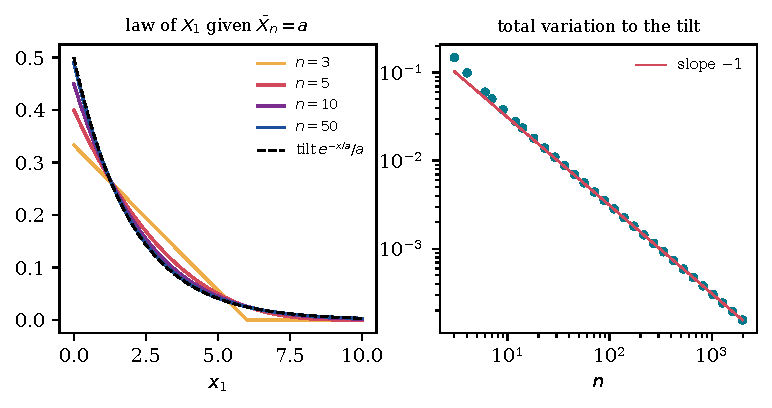
\includegraphics[width=\textwidth]{conditioning}
\caption{Moment conditioning. Left, the law of $X_1$ given $\bar X_n=2$ for independent standard exponentials, for $n=3,5,10,50$, with the exponential tilt (dashed). Right, the total variation distance to the tilt, which is the same for every mean, decays like $1/n$ with constant $c\approx0.31$.}
\label{fig:conditioning}
\end{figure}

\begin{proposition}[Poisson samples]
\label{prop:poisson}
Let $X_1,\dots,X_n$ be independent Poisson variables with mean one. Conditionally on $\sum_iX_i = N$, the vector is multinomial with $N$ trials and equal cell probabilities, so $X_1$ is Binomial$(N,1/n)$. If $N/n\to a$, this converges to the Poisson law with mean $a$, which is the exponential tilt $P_\lambda(x)\propto e^{\lambda x}\frac{e^{-1}}{x!}$ with $e^\lambda = a$.
\end{proposition}

\begin{proof}
The multinomial statement is the standard Poisson splitting identity read backwards, and the binomial to Poisson limit is classical.
\end{proof}

\section{Conditioning on collision invariants}

The equilibria of the Boltzmann equation are the Maxwellians, the densities whose logarithms are collision invariants, by the $H$ theorem (Theorem~\ref{thm:htheorem} of Chapter~\ref{ch:kinetic}). Moment conditioning gives them a second characterization: they are the laws of a single particle in a large system conditioned on its total mass, momentum and energy. Example~\ref{ex:maxwellian} of Chapter~\ref{ch:axioms} conditions on the energy alone; here the momentum is fixed as well, and the statement for $k$ particles comes with a rate.

\begin{theorem}[Moment conditioning produces Maxwellians]
\label{thm:maxwellian}
Let $V_1,\dots,V_n$ be independent standard Gaussian vectors in $\R^d$, and condition on
\[
\frac1n\sum_{i=1}^nV_i = u,\qquad\frac1n\sum_{i=1}^n|V_i-u|^2 = d\theta,
\]
with $u\in\R^d$ and $\theta>0$. The conditional law of $(V_1,\dots,V_n)$ is the uniform law on a sphere of radius $\sqrt{nd\theta}$ in an affine subspace of dimension $d(n-1)$, and the conditional law of $V_1$ converges in total variation to the Maxwellian $N(u,\theta I_d)$. For fixed $k$, the conditional law of $(V_1,\dots,V_k)$ converges to $N(u,\theta I_d)^{\otimes k}$.
\end{theorem}

\begin{proof}
Write $V_i = \bar V+W_i$ with $\bar V$ the mean and $\sum_iW_i = 0$. Under the Gaussian law $\bar V$ is independent of $(W_i)$, and $(W_i)$ is a standard Gaussian vector in the subspace $\{\sum_iw_i = 0\}$ of $(\R^d)^n$, of dimension $d(n-1)$. Conditioning fixes $\bar V = u$ and $\sum_i|W_i|^2 = nd\theta$, and by rotation invariance the conditional law of $(W_i)$ is uniform on the sphere of that radius in the subspace. The vector $W_1$ is the image of this uniform point under the linear map $w\mapsto w_1$, which is $\sqrt{(n-1)/n}$ times an orthogonal projection onto a $d$ dimensional subspace. By the Maxwell, Poincar\'e and Borel lemma (Theorem~\ref{thm:sphere_lemma} of Chapter~\ref{ch:poincare}), a $d$ dimensional projection of a uniform point on a sphere of dimension $d(n-1)-1$ and radius $\sqrt{nd\theta}$ is approximately Gaussian with covariance $\frac{nd\theta}{d(n-1)}I_d$, and multiplying by $\sqrt{(n-1)/n}$ gives covariance $\theta I_d$. Convergence in total variation follows from the explicit density as in that lemma. For $k$ particles, the map $w\mapsto(w_1,\dots,w_k)$ on the subspace has Gram matrix $(I_k-J_k/n)\otimes I_d$, where $J_k$ is the $k\times k$ matrix of ones, because $\sum_iw_i = 0$. It is therefore $B$ times a coisometry $U$ onto $\R^{kd}$, with $B = (I_k-J_k/n)^{1/2}\otimes I_d$, and $Uw$ consists of $kd$ orthonormal coordinates of a uniform point on a sphere of dimension $d(n-1)-1$. By Diaconis and Freedman~\cite{diaconisfreedman1987}, these coordinates are within total variation $(kd+3)/(d(n-1-k)-3)$ of the Gaussian law $N(0,\frac{n\theta}{n-1}I_{kd})$, and applying $B$ shows that $(W_1,\dots,W_k)$ is within the same distance of $N\big(0,\frac{n\theta}{n-1}(I_k-J_k/n)\otimes I_d\big)$. This covariance is not a multiple of the identity, because the velocities sum to $nu$, but its eigenvalues $\theta n/(n-1)$ and $\theta(n-k)/(n-1)$ are within $k\theta/(n-1)$ of $\theta$. The relative entropy between two centered Gaussian laws is half the sum of $\kappa-1-\log\kappa$ over the eigenvalues $\kappa$ of the ratio of their covariances, which is at most $\frac12\sum(\kappa-1)^2$ when all $\kappa\geq\frac12$, and Pinsker's inequality then shows that the two Gaussian laws are within total variation $k\sqrt d/n$ when $n\geq2k$. Hence the conditional law of $(V_1,\dots,V_k)$ is within total variation $O(kd/n)$ of $N(u,\theta I_d)^{\otimes k}$.
\end{proof}

Figure~\ref{fig:spheremaxwell} shows two velocity components of a uniform point on $S^{n-1}(\sqrt n)$. For $n = 3$ the mass concentrates near the rim of the disc, for $n = 6$ it fills the disc unevenly, and for $n = 60$ it is visibly the isotropic Gaussian.

\begin{figure}[t]
\centering
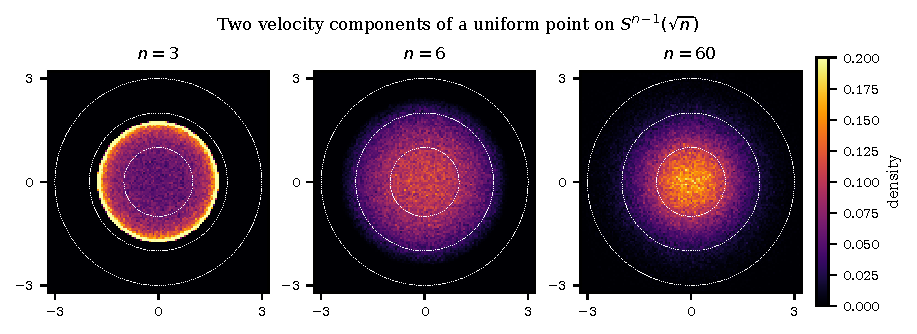
\includegraphics[width=\textwidth]{sphere_maxwell}
\caption{Joint density histogram of two coordinates of a uniform point on the sphere of radius $\sqrt{n}$ in $\R^n$, for $n=3$, $6$ and $60$ (left to right), from $200000$ points in each panel, on the square $[-3.2,3.2]^2$ and on one color scale (the bar at the right). The dotted circles of radius $1$, $2$ and $3$ are contours of the limiting standard Gaussian density. This is the energy shell of Theorem~\ref{thm:maxwellian} without the conditioning on the mean velocity. As $n$ grows the microcanonical law converges to the Maxwellian.}
\label{fig:spheremaxwell}
\end{figure}

The theorem has three readings. In kinetic theory it is the equivalence of ensembles~\cite{lanford1973,georgii1995}. In statistics it is the Bayesian statement that, after conditioning on sufficient statistics, the remaining randomness is uniform on the fiber, and its short marginals are approximately the fitted exponential family; this is the basis of conditional inference and of exact tests in exponential families. In the moment closure methods of Chapter~\ref{ch:kinetic}, it motivates Levermore's maximum entropy closure~\cite{levermore1996}: if a kinetic density is known only through finitely many moments, the conditional limit theorem selects the exponential family member with those moments as the most probable completion, which is Jaynes's maximum entropy choice~\cite{jaynes1957}. This is a heuristic and not a consequence, because the closure is a deterministic closure of a hierarchy of moment equations, whereas the theorem concerns independent particles conditioned on their moments.

\section{Bayes mixtures as universal codes}

The method of types also gives a short proof that a Bayes mixture is a good code for a family of sources. A code that assigns probability $M(x^n)$ to the binary sequence $x^n$ has length $-\log M(x^n)$, and its regret on $x^n$ is the excess of this length over the length achieved by the best Bernoulli model chosen with hindsight. We write $P_p^n(x^n) = p^k(1-p)^{n-k}$ for the probability of a sequence with $k$ ones under the Bernoulli law with parameter $p$.

\begin{theorem}[Laplace mixture]
\label{thm:laplacemixture}
Let $M(x^n) = \int_0^1p^k(1-p)^{n-k}\dd p$ be the marginal probability of a binary sequence with $k$ ones under the uniform prior. Then
\[
M(x^n) = \frac{1}{(n+1)\binom nk},\qquad-\log M(x^n)\leq n\,H\Big(\frac kn\Big)+\log(n+1).
\]
\end{theorem}

\begin{proof}
The Beta integral gives $\frac{k!(n-k)!}{(n+1)!}$, which is the first identity. By Theorem~\ref{thm:typecount}(3) with two letters, $\binom nk = |T(k/n)|\leq e^{nH(k/n)}$, which gives the bound.
\end{proof}

Since $nH(k/n) = -\log\max_p\,p^k(1-p)^{n-k}$, the Laplace mixture has regret at most $\log(n+1)$ uniformly over all sequences, and exactly $\log(n+1)$ on the two constant sequences. Its predictive law is Laplace's rule of succession~\cite{laplace1814}, derived in Section~\ref{sec:binary_definetti}, and the regret bound is also a bound on prediction. By the chain rule for relative entropy, $\E_p\log\frac{P_p^n(X^n)}{M(X^n)}$ is the sum over $i<n$ of the expected relative entropy between the Bernoulli law with parameter $p$ and the predictive law given $X^i$, and it is at most $\log(n+1)$ for every $p$, because $P_p^n(x^n)$ is at most the maximum over $p$. The average prediction error therefore tends to zero at rate $\log(n+1)/n$, uniformly in $p$, which is the information theoretic form of Bayesian consistency for this family.

Jeffreys' prior~\cite{jeffreys1946} for this family is Beta$(\frac12,\frac12)$, and its mixture is the Krichevsky Trofimov code~\cite{krichevsky1981}, which assigns probability $\Gamma(k+\frac12)\Gamma(n-k+\frac12)/(\pi\,\Gamma(n+1))$ to a sequence with $k$ ones. It does better than the uniform prior, with worst case regret $\frac12\log n+\frac12\log\pi+o(1)$, attained at the constant sequences (Exercise~\ref{ex:kt}). The smallest possible worst case regret is the minimax regret, and Shtarkov~\cite{shtarkov1987} identified the code that attains it. The normalized maximum likelihood code $\hat M(x^n) = \max_pP_p^n(x^n)/S_n$, with $S_n = \sum_{x^n}\max_pP_p^n(x^n) = \sum_{k=0}^n\binom nk(k/n)^k(1-k/n)^{n-k}$, has regret $\log S_n$ on every sequence, and every code has regret at least $\log S_n$ on some sequence, because a code with smaller regret on all sequences would give total probability more than one. By Stirling's formula $S_n = \sqrt{\pi n/2}\,(1+o(1))$, so that the minimax regret is $\frac12\log\frac{\pi n}{2}+o(1)$ (Exercise~\ref{ex:kt}), and the Krichevsky Trofimov mixture exceeds it by $\frac12\log2$, half a bit (Figure~\ref{fig:regret}).

The half bit comes from the boundary of the parameter space. For $k/n$ bounded away from $0$ and $1$ the Jeffreys mixture has regret $\frac12\log\frac{\pi n}{2}+o(1)$, the minimax value, and mixtures that add a small weight near the boundary attain the minimax regret asymptotically on every sequence, as Xie and Barron~\cite{xiebarron2000} showed. Jeffreys' prior, the reference prior of Bernardo~\cite{bernardo1979}, is optimal in another sense. The average over the prior of the expected redundancy $\E_p\log\frac{P_p^n(X^n)}{M(X^n)}$ is the mutual information between the parameter and the sample, and Clarke and Barron~\cite{clarkebarron1990,clarkebarron1994} showed that, over a compact set in the interior of the parameter space, Jeffreys' prior asymptotically maximizes it, that is, it is asymptotically least favorable, and that its mixture is asymptotically minimax for the expected redundancy.

For a smooth family of dimension $d$ the leading term of the regret is $\frac d2\log n$. Rissanen~\cite{rissanen1984} showed that, for every code and every $\varepsilon>0$, the set of parameter values at which the expected redundancy falls below $(1-\varepsilon)\frac d2\log n$ has Lebesgue measure tending to zero as $n$ grows, and for regular families $\frac d2\log n$ is also the leading term of the minimax regret~\cite{rissanen1996,xiebarron2000}. This is the minimum description length counterpart of the Bayesian information criterion~\cite{rissanen1978,schwarz1978}.

\begin{figure}[t]
\centering
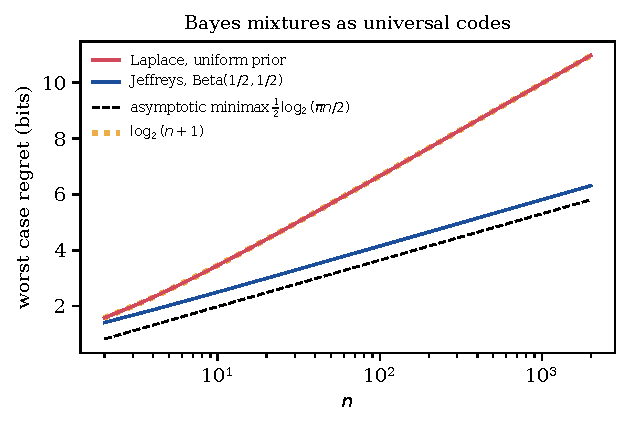
\includegraphics[width=0.85\textwidth]{regret}
\caption{Worst case regret, in bits, of the Laplace and Jeffreys mixtures for Bernoulli sequences. The Laplace curve coincides with the dotted curve $\log_2(n+1)$, which it attains at the constant sequences. The dashed curve is the asymptotic form $\frac12\log_2(\pi n/2)$ of the minimax regret of Shtarkov's code; the exact minimax regret is larger for small $n$ (for example $1.32$ bits against $0.83$ at $n=2$), and the Jeffreys curve lies half a bit above the dashed curve for large $n$.}
\label{fig:regret}
\end{figure}

\section{Hypothesis testing: Stein's lemma}

\begin{theorem}[Stein]
\label{thm:stein}
Let $X_1,\dots,X_n$ be independent with law $P_0$ under $H_0$ and $P_1$ under $H_1$, on a finite alphabet, with $P_0\ll P_1$. For $\varepsilon\in(0,1)$, let $\beta_n(\varepsilon)$ be the smallest type II error among tests with type I error at most $\varepsilon$. Then
\[
\lim_{n\to\infty}\frac1n\log\beta_n(\varepsilon) = -\KL(P_0\,\|\,P_1).
\]
\end{theorem}

\begin{proof}[Proof by types]
For the achievability, accept $H_0$ when $\KL(L_n\|P_0)\leq\delta$. Under $H_0$ this fails with probability at most $(n+1)^me^{-n\delta}$ by Theorem~\ref{thm:typecount}, so the type I error is at most $\varepsilon$ for large $n$. Under $H_1$ the acceptance probability is at most $(n+1)^m\exp(-n\min\{\KL(Q\|P_1):\KL(Q\|P_0)\leq\delta\})$, and the minimum tends to $\KL(P_0\|P_1)$ as $\delta\to0$: the minimizers converge to $P_0$ by Pinsker's inequality, and $\KL(\cdot\|P_1)$ is lower semicontinuous. For the converse, let $A_n$ be an acceptance region with $P_0^n(A_n)\geq1-\varepsilon$ and let $B_n$ be the set of $x\in A_n$ with $P_0^n(x)>0$ and $\KL(Q_x\|P_0)\leq\delta$. By the achievability computation $P_0^n(B_n)\geq(1-\varepsilon)/2$ for large $n$. For $x\in B_n$, Theorem~\ref{thm:typecount}(2) applied to $P_0$ and to $P_1$ gives
\[
\begin{aligned}P_1^n(x) &= P_0^n(x)\exp\Big(-n\sum_{a:P_0(a)>0}Q_x(a)\log\frac{P_0(a)}{P_1(a)}\Big)\\ &\geq P_0^n(x)e^{-n(\KL(P_0\|P_1)+\delta')},\end{aligned}
\]
where $\delta' = \sqrt{2\delta}\,\max_{P_0(a)>0}\big|\log\frac{P_0(a)}{P_1(a)}\big|$, because $Q_x\ll P_0\ll P_1$ and, by Pinsker's inequality, $\sum_a|Q_x(a)-P_0(a)|\leq\sqrt{2\delta}$. Hence $\beta_n\geq P_1^n(B_n)\geq\frac{1-\varepsilon}2e^{-n(\KL(P_0\|P_1)+\delta')}$, and letting $\delta\to0$ gives the lower bound on the exponent.
\end{proof}

If $P_0\not\ll P_1$, some letter $a$ has $P_0(a)>0 = P_1(a)$, and the test that accepts $H_0$ when $a$ occurs has type I error $(1-P_0(a))^n\to0$ and type II error zero, so that both sides of the theorem are $-\infty$. The theorem is the Chernoff Stein lemma~\cite{chernoff1956}; see Cover and Thomas~\cite[Section~11.8]{covertomas}.

Relative entropy is therefore the exponent of optimal discrimination, and the expected log likelihood ratio per observation, the quantity that drives the Bayes factor, is exactly this exponent. When one minimizes instead the average of the two error probabilities, the optimal exponent is the Chernoff information~\cite{chernoff1952} $C(P_0,P_1) = -\min_{0\leq s\leq1}\log\sum_xP_0(x)^sP_1(x)^{1-s}$, and the minimizing tilted law $P_s\propto P_0^sP_1^{1-s}$ is again an I projection, of $P_0$ onto the linear family $\{Q:\E_Q\log(P_1/P_0) = 0\}$ of laws equidistant in relative entropy from $P_0$ and $P_1$. Indeed, the derivative in $s$ of $\log\sum_xP_0^sP_1^{1-s}$ vanishes exactly when $\E_{P_s}\log(P_1/P_0) = 0$, and $P_s$ is a tilt of $P_0$, so that Theorem~\ref{thm:pythagoras} applies; moreover $C = \KL(P_s\|P_0) = \KL(P_s\|P_1)$ at the minimizing $s$ (Cover and Thomas~\cite[Section~11.9]{covertomas}).

\section{Types for Markov chains}

For a Markov chain on $\mathcal{X}$ with transition matrix $K$, the right notion of type is the pair type, the empirical distribution $Q^{(2)}$ of consecutive pairs $(x_i,x_{i+1})$, with first marginal $Q^{(1)}$. The two marginals of a pair type differ only through the first and last symbols of the sequence, so they agree up to $1/n$, and only pair types whose two marginals agree matter in the limit. Counting sequences with a given pair type uses an exact formula of Whittle~\cite{whittle1955} for the size of a pair type class, and the result, developed by Davisson, Longo and Sgarro~\cite{davisson1981} and by Csisz\'ar, Cover and Choi~\cite{csiszar1987}, is that the probability of a pair type with equal marginals decays, up to polynomial factors, at the rate
\[
I(Q^{(2)}) = \sum_{a,b}Q^{(2)}(a,b)\log\frac{Q^{(2)}(a,b)}{Q^{(1)}(a)K(a,b)},
\]
the relative entropy of the empirical transition law from the true one, averaged over the empirical marginal (see Csisz\'ar~\cite[Section~VII]{csiszar1998}). Contracting to the empirical marginal $\mu = Q^{(1)}$, that is, minimizing $I$ over the pair types whose two marginals equal $\mu$, gives the Donsker Varadhan rate function $-\inf_{u>0}\sum_a\mu(a)\log\frac{(Ku)(a)}{u(a)}$ of the occupation measure of the chain~\cite{donsker1975,dembozeitouni}. For a reversible process in continuous time, such as the Brownian motion of Chapter~\ref{ch:quantum}, the rate function is the Dirichlet form of $\sqrt{\dd\mu/\dd\pi}$, where $\pi$ is the invariant law, which connects large deviations with spectral gaps and, through Chapter~\ref{ch:ergodic}, with the efficiency of Monte Carlo. In discrete time the rate function is bounded below by the Dirichlet form $\frac12\sum_{a,b}\pi(a)K(a,b)\big(g(a)-g(b)\big)^2$ of $g = \sqrt{\mu/\pi}$, because $\log y\leq y-1$, but it is not equal to it: for the two state chain that flips with probability $0.3$ and $\mu = (0.2,0.8)$ the rate is $0.0851$ and the Dirichlet form is $0.0600$.

\section{Boltzmann's count revisited}

A gas of $n$ molecules whose one particle phase space is divided into $m$ cells has a type, the occupation vector divided by $n$. Under the uniform reference measure on cells, the number of microstates with type $Q$ is $|T(Q)|\approx e^{nH(Q)}$, Boltzmann's $W$. Conditioning on the total energy, a linear constraint on the type, selects with overwhelming probability the types near the I projection of the uniform law onto the energy shell, which is the Gibbs distribution, and by the conditional limit theorem the law of a single molecule converges to it, provided that the shell contains types, as when the cell energies are integers. Boltzmann's $H$ theorem~\cite{boltzmann1872}, read in this light, says that the collision dynamics carries the type of the gas toward the most numerous type compatible with the conserved quantities. This reading is ours and is not a theorem. Lanford's theorem~\cite{lanford1975} (Theorem~\ref{thm:lanford} of Chapter~\ref{ch:kinetic}) justifies the Boltzmann equation for hard spheres on a short time window, to which the $H$ theorem then applies, but it does not show that the type of the gas reaches the most numerous type, which would require the Boltzmann equation to hold over times long compared with the window, the subject of recent work of Deng, Hani and Ma~\cite{denghanima2024}. The method of types explains why the destination, if it is reached, is an exponential family.

\section*{Notes}

Csisz\'ar and K\"orner's \emph{Information Theory: Coding Theorems for Discrete Memoryless Systems}~\cite{csiszarkorner2011} develops the method of types systematically, and Csisz\'ar's survey \emph{The method of types}~\cite{csiszar1998} is a short introduction. Hoeffding~\cite{hoeffding1965} studies asymptotically optimal tests for multinomial distributions, the setting of Stein's lemma. Diaconis and Freedman~\cite{diaconisfreedman1988} give finite versions of conditional limit theorems for exponential families.

\section*{Exercises}
\begin{enumerate}
\item Prove that $|T(Q)| = n!/\prod_a(nQ(a))!$. Use Stirling's formula to show that $|T(Q)| = (2\pi n)^{-(m-1)/2}\prod_aQ(a)^{-1/2}e^{nH(Q)}(1+o(1))$ when $nQ(a)\to\infty$ for every $a$, and compare this with the bounds of Theorem~\ref{thm:typecount}(3), which hold for every type.
\item Compute the I projection of the uniform law on $\{1,\dots,6\}$ onto $\{Q:\E_Qx = 4.5\}$, Jaynes's Brandeis dice problem~\cite{jaynes1963}, and verify the Pythagorean identity numerically. The projection is $P^*(x)\propto e^{\lambda x}$ with $\lambda\approx0.371$.
\item\label{ex:ipf} Let $P$ be a law with full support on $\{1,\dots,m\}\times\{1,\dots,m'\}$ and let $r$ and $c$ be laws with full support on the two factors. Let $\pi_0 = P$, let $\pi_{t+1}$ be $\pi_t$ with its rows rescaled to have sums $r$ when $t$ is even, and with its columns rescaled to have sums $c$ when $t$ is odd (iterative proportional fitting), and let $\pi^*$ be the I projection of $P$ onto the laws with marginals $r$ and $c$. Show that rescaling the rows is the I projection onto the laws with first marginal $r$, and likewise for the columns. Show that $\KL(\pi^*\|\pi_t)$ decreases at each step, using the Pythagorean identity. Show by an example that $\KL(\pi_t\|\pi^*)$ need not decrease: for $P = \frac19\begin{pmatrix}3&2\\1&3\end{pmatrix}$, $r = (\frac12,\frac12)$ and $c = (\frac78,\frac18)$, it rises from $0.621$ to $0.625$ at the first step, while $\KL(\pi^*\|\pi_t)$ falls from $0.506$ to $0.499$.
\item Verify the exact conditional density of the exponential example and the value of the constant $c$ in its total variation rate.
\item\label{ex:kt} Show that the Krichevsky Trofimov mixture assigns probability $\frac{\Gamma(k+\frac12)\Gamma(n-k+\frac12)}{\pi\,\Gamma(n+1)}$ to a sequence with $k$ ones, and derive its worst case regret. Show that the regret is largest on the constant sequences, where it is $\frac12\log(\pi n)+o(1)$ (treat $k$ as a continuous variable and use $\psi'(x+\frac12)<1/x$ for the digamma function $\psi$), and that Shtarkov's sum satisfies $S_n = \sqrt{\pi n/2}\,(1+o(1))$ by Stirling's formula.
\item Compute the Chernoff information between $\mathrm{Bernoulli}(p)$ and $\mathrm{Bernoulli}(q)$ and the optimal tilting parameter.
\end{enumerate}
